%%
%% This is file `sample-acmsmall-submission.tex',
%% generated with the docstrip utility.
%%
%% The original source files were:
%%
%% samples.dtx  (with options: `acmsmall-submission')
%% 
%% IMPORTANT NOTICE:
%% 
%% For the copyright see the source file.
%% 
%% Any modified versions of this file must be renamed
%% with new filenames distinct from sample-acmsmall-submission.tex.
%% 
%% For distribution of the original source see the terms
%% for copying and modification in the file samples.dtx.
%% 
%% This generated file may be distributed as long as the
%% original source files, as listed above, are part of the
%% same distribution. (The sources need not necessarily be
%% in the same archive or directory.)
%%
%% The first command in your LaTeX source must be the \documentclass command.
\documentclass[sigconf,review,anonymous]{acmart}
\usepackage{url}
\usepackage{todonotes}
\usepackage{listings}
%%
%% \BibTeX command to typeset BibTeX logo in the docs
\AtBeginDocument{%
  \providecommand\BibTeX{{%
    \normalfont B\kern-0.5em{\scshape i\kern-0.25em b}\kern-0.8em\TeX}}}

%% Rights management information.  This information is sent to you
%% when you complete the rights form.  These commands have SAMPLE
%% values in them; it is your responsibility as an author to replace
%% the commands and values with those provided to you when you
%% complete the rights form.
\setcopyright{acmcopyright}
\copyrightyear{2018}
\acmYear{2018}
\acmDOI{10.1145/1122445.1122456}


%%
%% These commands are for a JOURNAL article.
\acmJournal{JACM}
\acmVolume{37}
\acmNumber{4}
\acmArticle{111}
\acmMonth{8}

%%
%% Submission ID.
%% Use this when submitting an article to a sponsored event. You'll
%% receive a unique submission ID from the organizers
%% of the event, and this ID should be used as the parameter to this command.
%%\acmSubmissionID{123-A56-BU3}

%%
%% The majority of ACM publications use numbered citations and
%% references.  The command \citestyle{authoryear} switches to the
%% "author year" style.
%%
%% If you are preparing content for an event
%% sponsored by ACM SIGGRAPH, you must use the "author year" style of
%% citations and references.
%% Uncommenting
%% the next command will enable that style.
%%\citestyle{acmauthoryear}

%%
%% end of the preamble, start of the body of the document source.
\begin{document}

%%
%% The "title" command has an optional parameter,
%% allowing the author to define a "short title" to be used in page headers.
\title{single statement bugs in dynamic language features}

%%
%% The "author" command and its associated commands are used to define
%% the authors and their affiliations.
%% Of note is the shared affiliation of the first two authors, and the
%% "authornote" and "authornotemark" commands
%% used to denote shared contribution to the research.
\author{Ben Trovato}
\authornote{Both authors contributed equally to this research.}
\email{trovato@corporation.com}
\orcid{1234-5678-9012}
\author{G.K.M. Tobin}
\authornotemark[1]
\email{webmaster@marysville-ohio.com}
\affiliation{%
  \institution{Institute for Clarity in Documentation}
  \streetaddress{P.O. Box 1212}
  \city{Dublin}
  \state{Ohio}
  \country{USA}
  \postcode{43017-6221}
}

\author{Lars Th{\o}rv{\"a}ld}
\affiliation{%
  \institution{The Th{\o}rv{\"a}ld Group}
  \streetaddress{1 Th{\o}rv{\"a}ld Circle}
  \city{Hekla}
  \country{Iceland}}
\email{larst@affiliation.org}

\author{Valerie B\'eranger}
\affiliation{%
  \institution{Inria Paris-Rocquencourt}
  \city{Rocquencourt}
  \country{France}
}


%%
%% By default, the full list of authors will be used in the page
%% headers. Often, this list is too long, and will overlap
%% other information printed in the page headers. This command allows
%% the author to define a more concise list
%% of authors' names for this purpose.
\renewcommand{\shortauthors}{Trovato and Tobin, et al.}

%%
%% The abstract is a short summary of the work to be presented in the
%% article.
\begin{abstract}
	TODO:
\end{abstract}

%%
%% The code below is generated by the tool at http://dl.acm.org/ccs.cfm.
%% Please copy and paste the code instead of the example below.
%%
% \begin{CCSXML}
% <ccs2012>
%  <concept>
%   <concept_id>10010520.10010553.10010562</concept_id>
%   <concept_desc>Computer systems organization~Embedded systems</concept_desc>
%   <concept_significance>500</concept_significance>
%  </concept>
%  <concept>
%   <concept_id>10010520.10010575.10010755</concept_id>
%   <concept_desc>Computer systems organization~Redundancy</concept_desc>
%   <concept_significance>300</concept_significance>
%  </concept>
%  <concept>
%   <concept_id>10010520.10010553.10010554</concept_id>
%   <concept_desc>Computer systems organization~Robotics</concept_desc>
%   <concept_significance>100</concept_significance>
%  </concept>
%  <concept>
%   <concept_id>10003033.10003083.10003095</concept_id>
%   <concept_desc>Networks~Network reliability</concept_desc>
%   <concept_significance>100</concept_significance>
%  </concept>
% </ccs2012>
% \end{CCSXML}

\ccsdesc[500]{Empirical software engineering,}
\ccsdesc[300]{Program analysis}
\ccsdesc{Java reflection}
\ccsdesc[100]{Bug detection}

%%
%% Keywords. The author(s) should pick words that accurately describe
%% the work being presented. Separate the keywords with commas.
% \keywords{Empirical software engineering, Program analysis, Java reflection, Bug detection}


%%
%% This command processes the author and affiliation and title
%% information and builds the first part of the formatted document.
\maketitle

\section{Introduction}


\section{Background}



\section{Methodology}
We discuss the methodology used in our study in this section. Figure \ref{fig:process} demonstrates an overview of process. The main dataset we used are from the SStuBs study \cite{karampatsis2020often}. Addition to the original SStuBs \cite{karampatsis2020often} dataset, we extend the dataset by including more projects from software communities on GitHub in order to obtain more dynamic language feature related bugs. These software communities include: Google\footnote{\url{https://github.com/google} [accessed on 12,May 2021]}, Eclipse\footnote{\url{https://github.com/eclipse} [accessed on 12,May 2021]}, Jetbrains\footnote{\url{https://github.com/JetBrains}}, Mozilla\footnote{\url{https://github.com/mozilla}}, Apache\footnote{\url{https://github.com/apache} [accessed on 12,May 2021]} and Spring\footnote{\url{https://github.com/spring-projects} [accessed on 12,May 2021]}. We select those communities based on the following criteria: 

\begin{itemize}
\item they have numbers of well-known Java projects.
\item all of projects are currently active and constantly updated.
\item communities that have issue tracking system, either be GitHub issue or other system such as bugzilla \footnote{\url{https://www.bugzilla.org/}} for Apache projects
\item projects that are known for using dynamic features, such as Spring.
\end{itemize}

\begin{figure}[H]
  \centering
      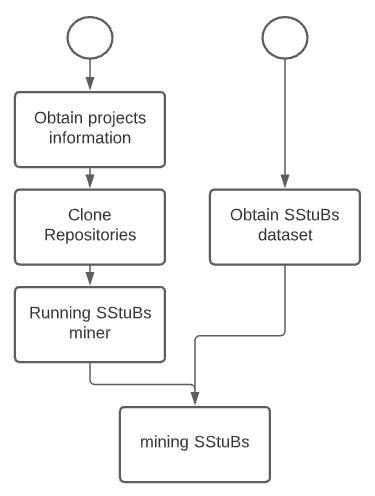
\includegraphics[width=0.7\columnwidth]{figures/process.png}
  \caption{an overview of process}
  \label{fig:process}
\end{figure}


Those 6 communities have quite numbers of projects so we need to harvest the url for each project in order to clone the repository. We use HTTP GET requests to retrieve community pages, which contain a list of projects. Then we use the Jsoup\footnote{\url{https://jsoup.org} [accessed on 12,May 2021]}: a HTML parser to retrieved HTML DOM that contains project urls. At this stage, we remove some projects that have been included the original SStuBs dataset to avoid duplications. Then all project are cloned to the local disk.  
%%explain why not use GitHub API, because we aim upto date project with latest commits and issues
The script that is then used to obtain single statement bugs from each cloned repository is provided by the SStuBs study\footnote{\url{https://github.com/mast-group/mineSStuBs} [accessed on 12,May 2021]}.  Once we have both datasets (original SStuBs and additional datasets from selected software communities), we use a script to identify single statement bugs that relate to dynamic features. To be precise to what we refer as dynamic language features, we select keywords from callsites to locate changes in the fix commits.  Those keywords are provided in Table \ref{tab:keyword}. We select those key words based on Sui et al.\cite{sui2018soundness}

\begin{table}[h]
\scriptsize
\caption{keywords}
\label{tab:keyword}
\footnotesize
\begin{tabular}{|l|p{5cm}|}
\hline
keyword                  & full name                    \\ \hline
.invoke(                 & java.lang.reflect.Method.invoke \\ \hline
.getDeclaredMethod(      & java.lang.Class.getDeclaredMethod\\ \hline
.getDeclaredConstructor( & java.lang.Class.getDeclaredConstructor\\ \hline
.getDeclaredField(       & java.lang.Class.getDeclaredField \\ \hline
.newInstance(            & java.lang.Class.newIstance\&java.lang.reflect.Constructor.newInstance\\ \hline
.forName(                & java.lang.Class.forName         \\ \hline
.findClass(              & java.lang.ClassLoader.findClass  \\ \hline
.defineClass(            & java.lang.ClassLoader.defineClass \\ \hline
.loadClass(              & java.lang.ClassLoader.loadClass   \\ \hline
.readObject(             & java.io.ObjectInputStream.readObject \\ \hline
.allocateInstance(       & sun.misc.Unsafe.allocateInstance     \\ \hline
.getInvocationHandler(   & java.lang.reflect.Proxy.getInvocationHandler\\ \hline
.newProxyInstance(       & java.lang.reflect.Proxy.newProxyInstance    \\ \hline
.load(                   & java.util.ServiceLoader.load           \\ \hline
\end{tabular}
\end{table}

\section{Results and Discussion}



\section{Conclusion}



% \section{Acknowledgments}



%%
%% The acknowledgments section is defined using the "acks" environment
%% (and NOT an unnumbered section). This ensures the proper
%% identification of the section in the article metadata, and the
%% consistent spelling of the heading.
% \begin{acks}
% To Robert, for the bagels and explaining CMYK and color spaces.
% \end{acks}

%%
%% The next two lines define the bibliography style to be used, and
%% the bibliography file.
\bibliographystyle{ACM-Reference-Format}
\bibliography{ref}

%%
%% If your work has an appendix, this is the place to put it.


\end{document}
\endinput
%%
%% End of file `sample-acmsmall-submission.tex'.
